\documentclass[10pt,showpacs,preprintnumbers,amsmath,amssymb,nofootinbib,aps,prl,twocolumn,groupedaddress,superscriptaddress,showkeys]{revtex4-1}
\usepackage{graphicx}
\usepackage{dcolumn}
\usepackage{bm}
\usepackage[colorlinks=true,urlcolor=blue,citecolor=blue]{hyperref}
\usepackage{color}
\usepackage{listings}
\usepackage{subfig}
\usepackage{float}
\usepackage{tikz} % Send help 
  \usetikzlibrary{automata, positioning}
\usepackage{physics}


\lstset{ %
  basicstyle=\footnotesize,        % the size of the fonts that are used for the code
  breakatwhitespace=false,         % sets if automatic breaks should only happen at whitespace
  breaklines=true,                 % sets automatic line breaking
  captionpos=t,                    % sets the caption-position to bottom
  deletekeywords={...},            % if you want to delete keywords from the given language
  escapeinside={\%*}{*)},          % if you want to add LaTeX within your code
  extendedchars=true,              % lets you use non-ASCII characters; for 8-bits encodings only, does not work with UTF-8
  frame=single,                    % adds a frame around the code
  keepspaces=true,                 % keeps spaces in text, useful for keeping indentation of code (possibly needs columns=flexible)
 % language=Python,                 % the language of the code
  morekeywords={*,...},           % if you want to add more keywords to the set
  numbers=left,                    % where to put the line-numbers; possible values are (none, left, right)
  numbersep=5pt,                   % how far the line-numbers are from the code
  showspaces=false,                % show spaces everywhere adding particular underscores; it overrides 'showstringspaces'
  showstringspaces=false,          % underline spaces within strings only
  showtabs=false,                  % show tabs within strings adding particular underscores
  stepnumber=1,                    % the step between two line-numbers. If it's 1, each line will be numbered
  tabsize=2,                       % sets default tabsize to 2 spaces
}

\newcommand{\lexp}{\ket{\downarrow}}
\begin{document}
\title{Disease Modeling - FYS3150 Computational Physics}
\author{Nicholas Karlsen}


\begin{abstract}
\end{abstract}

\maketitle


\section{Introduction}

\section{Theory, Algorithms and Methods}  
  \subsection{Runge-Kutta methods}
    

  \subsection{\label{sec:Markov Chains}Markov Chains}
    A Markov Chain aims to model the behavior of stochastic processes, that is models which time-evolution of each parameter $x_i$ is governed by a set of transition probabilities $P(x_i \rightarrow x_j)$.

    The k-th state of the system is given by the state vector $\vb x_k$, a column vector with entries $x_i$ for each parameter of the system.
      \begin{equation}
        \vb x_k = \mqty(x_1 \\ \vdots \\ x_i \\ \vdots \\ x_n)
      \end{equation}
    The transition probabilities $P(x_i\rightarrow x_j)$ are contained within a Stochastic matrix, $M$, an $n\times n$ matrix which columns are probability vectors that sum to unity. $M$ is such that multiplying it by a state $\vb x_k$ determines the next state, $\vb x_{k+1}$
      \begin{equation}
        M \vb x_k = \vb x_{k+1}
      \end{equation}

    From Theorem 18 in \textcite[p.~277]{linalg_lays}, if $M$ is a regular stochastic matrix there exists a unique steady state vector $\vb q$ which the system will converge towards as $k\rightarrow \infty$ characterized by
    \begin{equation}
      \vb x_k = \vb x_{k+1} 
    \end{equation}
    Regardless of the initial state, $\vb x_0$.

  \subsection{SIRS Model}

    The SIRS model is a type of mathematical model describing how infectious disease evolves within a population, and is a part of a family of similar models in epidemiology with various different features. In the SIRS model, the total population (N) is divided into three groups

    \begin{itemize}
      \item Susceptible (S) : People who do not have the disease, and are not immune to it.
      \item Infected (I) : People who are infected with the disease.
      \item Recovered (R) : People who has recovered from the infection, and have developed immunity.
    \end{itemize}

    Where the permitted traversal from one group to another follows a cyclical pattern $S \rightarrow I \rightarrow R \rightarrow S$.

    The rate of traversal is governed by a set of coupled differential equations,

    \begin{align}
      \begin{split}
        S' &= cR - \frac{aSI}{N} \\
        I' &= \frac{aSI}{N} - bI \\
        R' &= bI - cR 
        \label{eqn:transition rates}
      \end{split}
    \end{align}
    Where the constants $a,b,c$ are governing the

    \begin{itemize}
      \item rate of transmission
      \item rate of recovery
      \item rate of immunity loss
    \end{itemize}

    respectively, with dimension inverse time. For the purposes of this report, we will not consider a specific unit of time, but rather the dynamics of the system, as the timescales at which different diseases operate on vary. However, based on data (INSERT CITATIONS) a lot of common diseases are observed to operate on a scale of days, whilst some operate on a scale of years. 

    This system can also be modelled as a Stochastic system described as a Markov Chain, shown as a Markov diagram in Fig.~\ref{fig:SIRS diagram}. If we consider a small, finite timeinterval $\Delta t$, we can approximate the transition probabilities $P(x_i \rightarrow x_j)$ from Eqn.~\ref{eqn:transition rates}

    \begin{align}
      \begin{split}
        P(S\rightarrow I) &= \frac{aSI}{N}\Delta t
          \\
        P(I\rightarrow R) &= bI\Delta t
          \\
        P(R\rightarrow S) &= cR\Delta t
      \end{split}
    \end{align}
    It follows then, that the system will reach a steady state after a finite number of transitions for any set of initial conditions as discussed in Section~\ref{sec:Markov Chains}

    \begin{figure}[h!tb]
      \centering 
      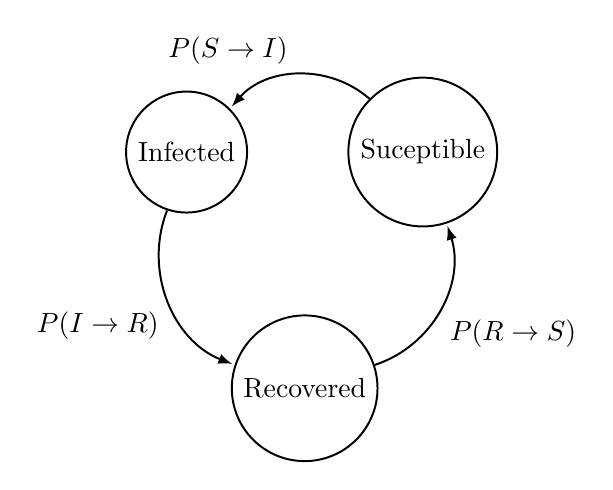
\begin{tikzpicture}
 
        % Setup the style for the states
        \tikzset{node style/.style={state, 
                                    minimum width=1.5cm,
                                    line width=.25mm
                                    }}
 
        % Draw the states
        \node[node style] at (3, 0)     (Suceptible)     {Suceptible};
        \node[node style] at (0, 0)     (Infected)     {Infected};
        \node[node style] at (1.5, -3) (Recovered) {Recovered};
 
        % Connect the states with arrows
        \draw[every loop,
              auto=right,
              line width=.25mm,
              >=latex]
            (Suceptible)    edge[bend right=45]  node {$P(S\rightarrow I)$} (Infected)
            (Infected)      edge[bend right=45]  node {$P(I\rightarrow R)$} (Recovered)
            (Recovered)     edge[bend right=45]  node {$P(R\rightarrow S)$} (Suceptible);
      \end{tikzpicture}
       \caption{The SIRS Model\label{fig:SIRS diagram}}
    \end{figure}



\section{Results and Discussions}

\section{Conclusions}


\bibliography{../bibliography.bib}


\end{document}  